% LaTeX Template for short student reports.
% Citations should be in bibtex format and go in references.bib

\begin{filecontents*}{\jobname.bib}
@preamble{"\DeclareRobustCommand{\firstsecond}[2]{#2}"}

@misc{Kaggle:2021,
  author = {{\firstsecond{Josh}{Joshua Swords}}},
  title = {HR Analytics: Job Change of Data Scientists},
  year = {2021},
  note = {data retrieved from Kaggle, 
          \url{https://www.kaggle.com/code/joshuaswords/awesome-hr-data-visualization-prediction/data}},
}
\end{filecontents*}



\documentclass[11pt]{article}
\usepackage[top=3cm, bottom=3cm, left = 2cm, right = 2cm]{geometry}  
\usepackage[utf8]{inputenc}
\usepackage{textcomp}
\usepackage{graphicx} 
\graphicspath{ {images/} }
\usepackage{wrapfig}
\usepackage{amsmath,amssymb}  
\usepackage{bm}  
\usepackage[pdftex,bookmarks,colorlinks,breaklinks]{hyperref}  
\hypersetup{linkcolor=black,citecolor=black,filecolor=black,urlcolor=blue} % black links, for printed output
\usepackage{memhfixc} 
\usepackage{pdfsync}  
\usepackage{fancyhdr}
\usepackage{indentfirst}
\usepackage[affil-it]{authblk}

\DeclareRobustCommand{\firstsecond}[2]{#1}

\renewcommand\Affilfont{\fontsize{9}{10.8}\itshape}
\pagestyle{fancy}

\title{Responsible Data Science Course Project}
\author{Claire Saint-Donat, Xiangyue Wang}
\affil{Center for Data Science, New York University}
\date{Spring 2022}

\begin{document}
\maketitle
\tableofcontents

\section{Introduction}

The purpose of this project is to build an interpretability tool for an Automated Decision System (ADS) which we have chosen to audit.

Automated Decision Systems are in widespread use in government and industry, and a number of efforts are currently underway to regulate them.  New York City recently passed a law (Local Law 49 of 2018) that compels the development of procedures and recommendations that City agencies should follow when explaining the operation of an ADS to the public, and demonstrating that an ADS does not discriminate against individuals based on membership in protected groups.  

In this project, we attempt to help NYC and other municipalities by designing a``nutritional label" (similar to a label used to evaluate food products) for an algorithmic system of our choice. 
\pagebreak

\section{Background}
In recent years, the growing demands for jobs in data science have driven the creation of a myriad of degree programs, massive online open courses, online certification programs, and boot camps. While the abundance of those learning resources has made data science accessible to a wide range of people looking to enter the field, the variety of credentials has also made it difficult for companies to evaluate the qualifications of job seekers. The process of hiring data scientists is often both expensive and time-consuming. Therefore, companies have incentives to hire qualified data scientists and keep them from leaving. 

As as a result of this trend, the Automated Decision System (ADS) that we chose to examine is from the Human Resources and hiring space.  In particular, we wish to examine a top entry from an HR Analytics Kaggle competition published \href{https://www.kaggle.com/code/joshuaswords/awesome-hr-data-visualization-prediction/notebook}{here}.  The source of these data come from a company active in the big data and data science industries that is looking to hire data scientists amongst a group of candidates who have taken training courses hosted by the company.  Many candidates sign up for training and the firm would like to know which trainees would be interested in working for the company and which are currently looking for new employment.  Targeting these candidates reduces costs and time associated with hiring data scientists.  In addition, a model of this kind would also help improve the quality of these trainings and the planning of courses that might further help categorize candidates in the future.  The desired outcome of this model is to accurately predict the probability that a given trainee is on the job market and is actively looking for a new position.  The ultimate action taken as a result of this ADS is determining which trainees should be invited to interview for data science positions at the company.

In the course of our analysis, we will examine these data, the cleaning process, and the system itself in order to evaluate whether the ADS discriminates on the basis of gender or socioeconomic status. If present, such discrimination could result in certain groups of employees receiving less rigorous training, fewer promotions and denied access to other benefits. Our aim is to design a ``nutritional label" for the ADS that examines the bias in the data, the processing, and one machine learning model used in this decision\-making process. 


\pagebreak

\section{Input and Output}

These data, made available by the company, are designed to understand the factors that lead a data scientist to search for a new job.  Important information pertaining to demographics, education and prior experience is made available (on an anonymized basis) from registered and enrolled candidates.  There is little information available about the geography of the candidate population in question or even the time during which these data were collected however we can discern from that they represent job candidates from 123 different cities of varying levels of development.  The total dataset for the ADS comprises 19,158 candidates with the following 14 features describing each:


\begin{table}[h]
\centering
\begin{tabular}{ |p{4cm}||p{10cm}|  }
 
 \hline
 Feature 		& Description		\\
 \hline
enrollee\_id 	& Unique ID for candidate\\
city			& Code given for candidate's city \\
city\_development\_index & Development index of the city (scaled)\\
gender		& Gender of candidate\\
relevant\_experience & Relevant experience of candidate\\
enrolled\_university & Type of University course enrolled if any \\

education\_level & Education level of candidate\\

major\_discipline & Education major discipline of candidate \\

experience 	& Candidate total experience in years\\

company\_size 	& Number of employees in current employer's company \\

company\_type 	& Type of current employer\\

last\_new\_job 	& Difference in years between previous job and current job \\

training\_hours 	& training hours completed \\

target 		& 0 - Not looking for job change, 1 – Looking for a job change\\
 \hline
\end{tabular}
\end{table}


%\begin{wrapfigure}{r}{0.45\textwidth}
%    \centering
%    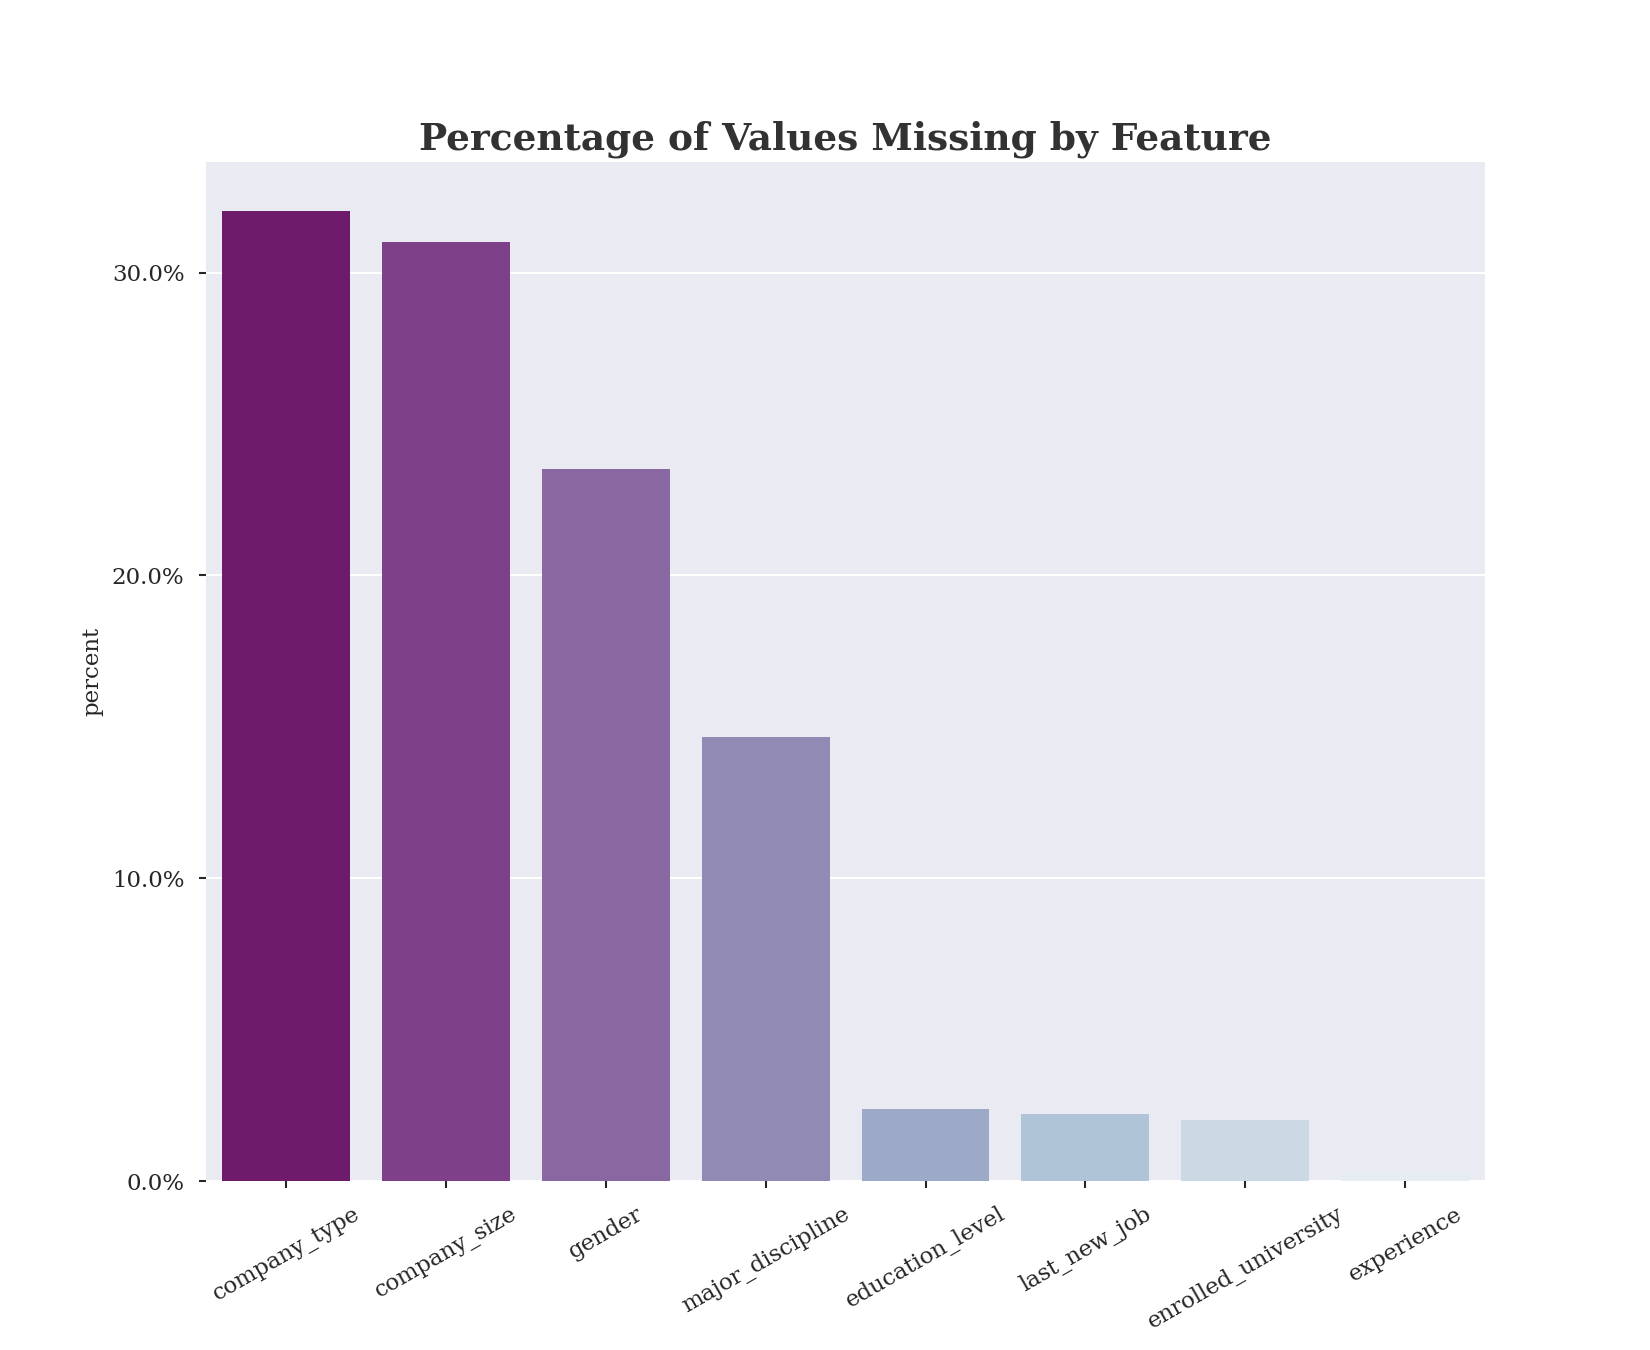
\includegraphics[width=0.45\textwidth]{missing_values}
%\end{wrapfigure}

\begin{center}
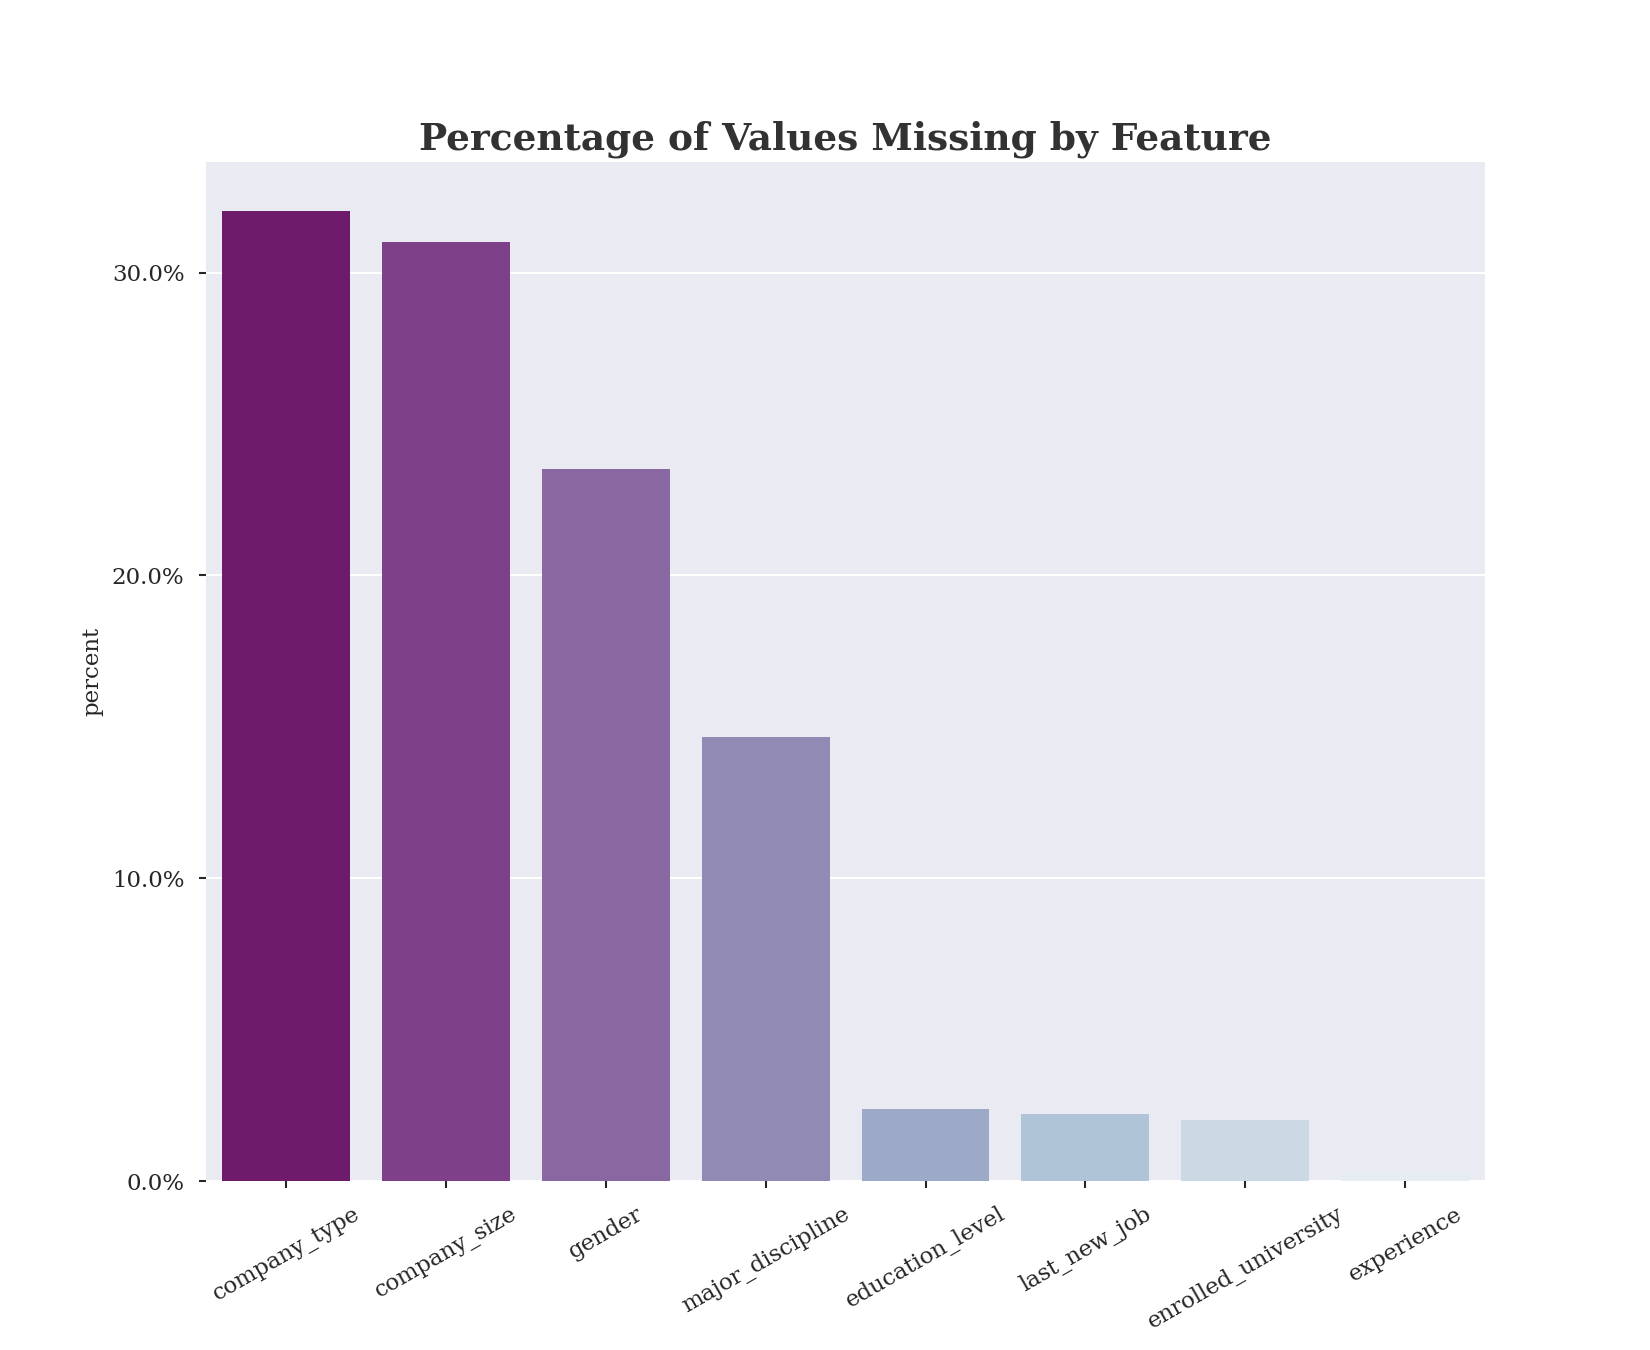
\includegraphics[width=0.45\textwidth]{missing_values}
\end{center}

The majority of these features are categorical(Nominal, Ordinal, Binary), some with high cardinality. The exceptions are \emph{city\_development\_index} and \emph{training hours} both of which are numeric. Some features have large proportions of missing values, particularly \emph{company\_type}, \emph{company\_size} and \emph{gender}.

\vspace{250px}



\begin{table}[h]
\centering
\begin{tabular}{ |p{4cm}||p{2cm}| p{2.53cm}| p{1.5cm}|}
 \hline
 Feature 		& Data Type	& Distinct Values	& \% Null\\
 \hline
enrollee\_id 	& int64 & 19,158 & 0.0 \%	\\
city			 & object & 123 & 0.0 \% \\
city\_development\_index & float64 & 93 & 0.0 \% \\
gender		& object & 4 & 23.5 \% \\
relevant\_experience & object & 2 & 0.0 \%\\

enrolled\_university & object & 4 & 2.0 \% \\

education\_level & object & 6 & 2.4 \% \\

major\_discipline  & object & 7 & 14.7 \% \\

experience  	& object & 23 & 0.7 \% \\

company\_size 	& object & 9 & 31.0 \% \\

company\_type 	& object & 7 & 32.0 \%\\

last\_new\_job 	& object & 7 & 2.2 \%\\

training\_hours & int64 & 241 & 0.0 \%  \\

target 		 & int64 & 2 & 0.0 \% \\
 \hline
\end{tabular}
\end{table}


In terms of relative distributions, this dataset is largely imbalanced on our target variable with 75\% of candidates not seeking a new job and only 25\% actively on the job market.  This imbalance is significant in that it will impact the choice of modeling and necessary data preparation steps of the decision system.

\begin{wrapfigure}{l}{0.45\textwidth}
    \centering
    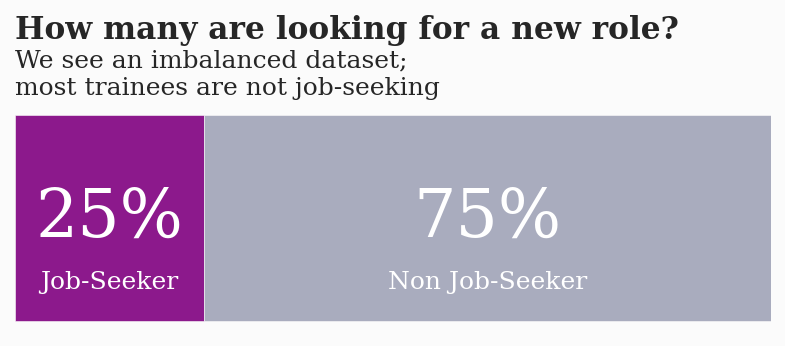
\includegraphics[width=0.45\textwidth]{download}
\end{wrapfigure}

%\vspace{2px}


\vspace{10px}
The overwhelming majority of candidates in the dataset are male, representing nearly 70\% of the total population. Similarly the majority of trainees have prior data science experience and at least an undergraduate degree in a STEM field.  The candidate pool is also largely experienced in the workforce with 60\% having 10 or more years of experience. The majority of candidates competed 47 hours of training or less with a long right tail.  While a large portion of candidates come from cities with development indices, there is another pool of candidates that comes from cities with an index just above 0.6. The full set of distribution plots and exploratory data analysis of each feature in the dataset can be found \href{https://github.com/cas2247/RDS_Algorithmic_Fairness/blob/main/notebooks/1_Input_and_Output.ipynb}{here}.


\begin{wrapfigure}{r}{0.45\textwidth}
    \centering
    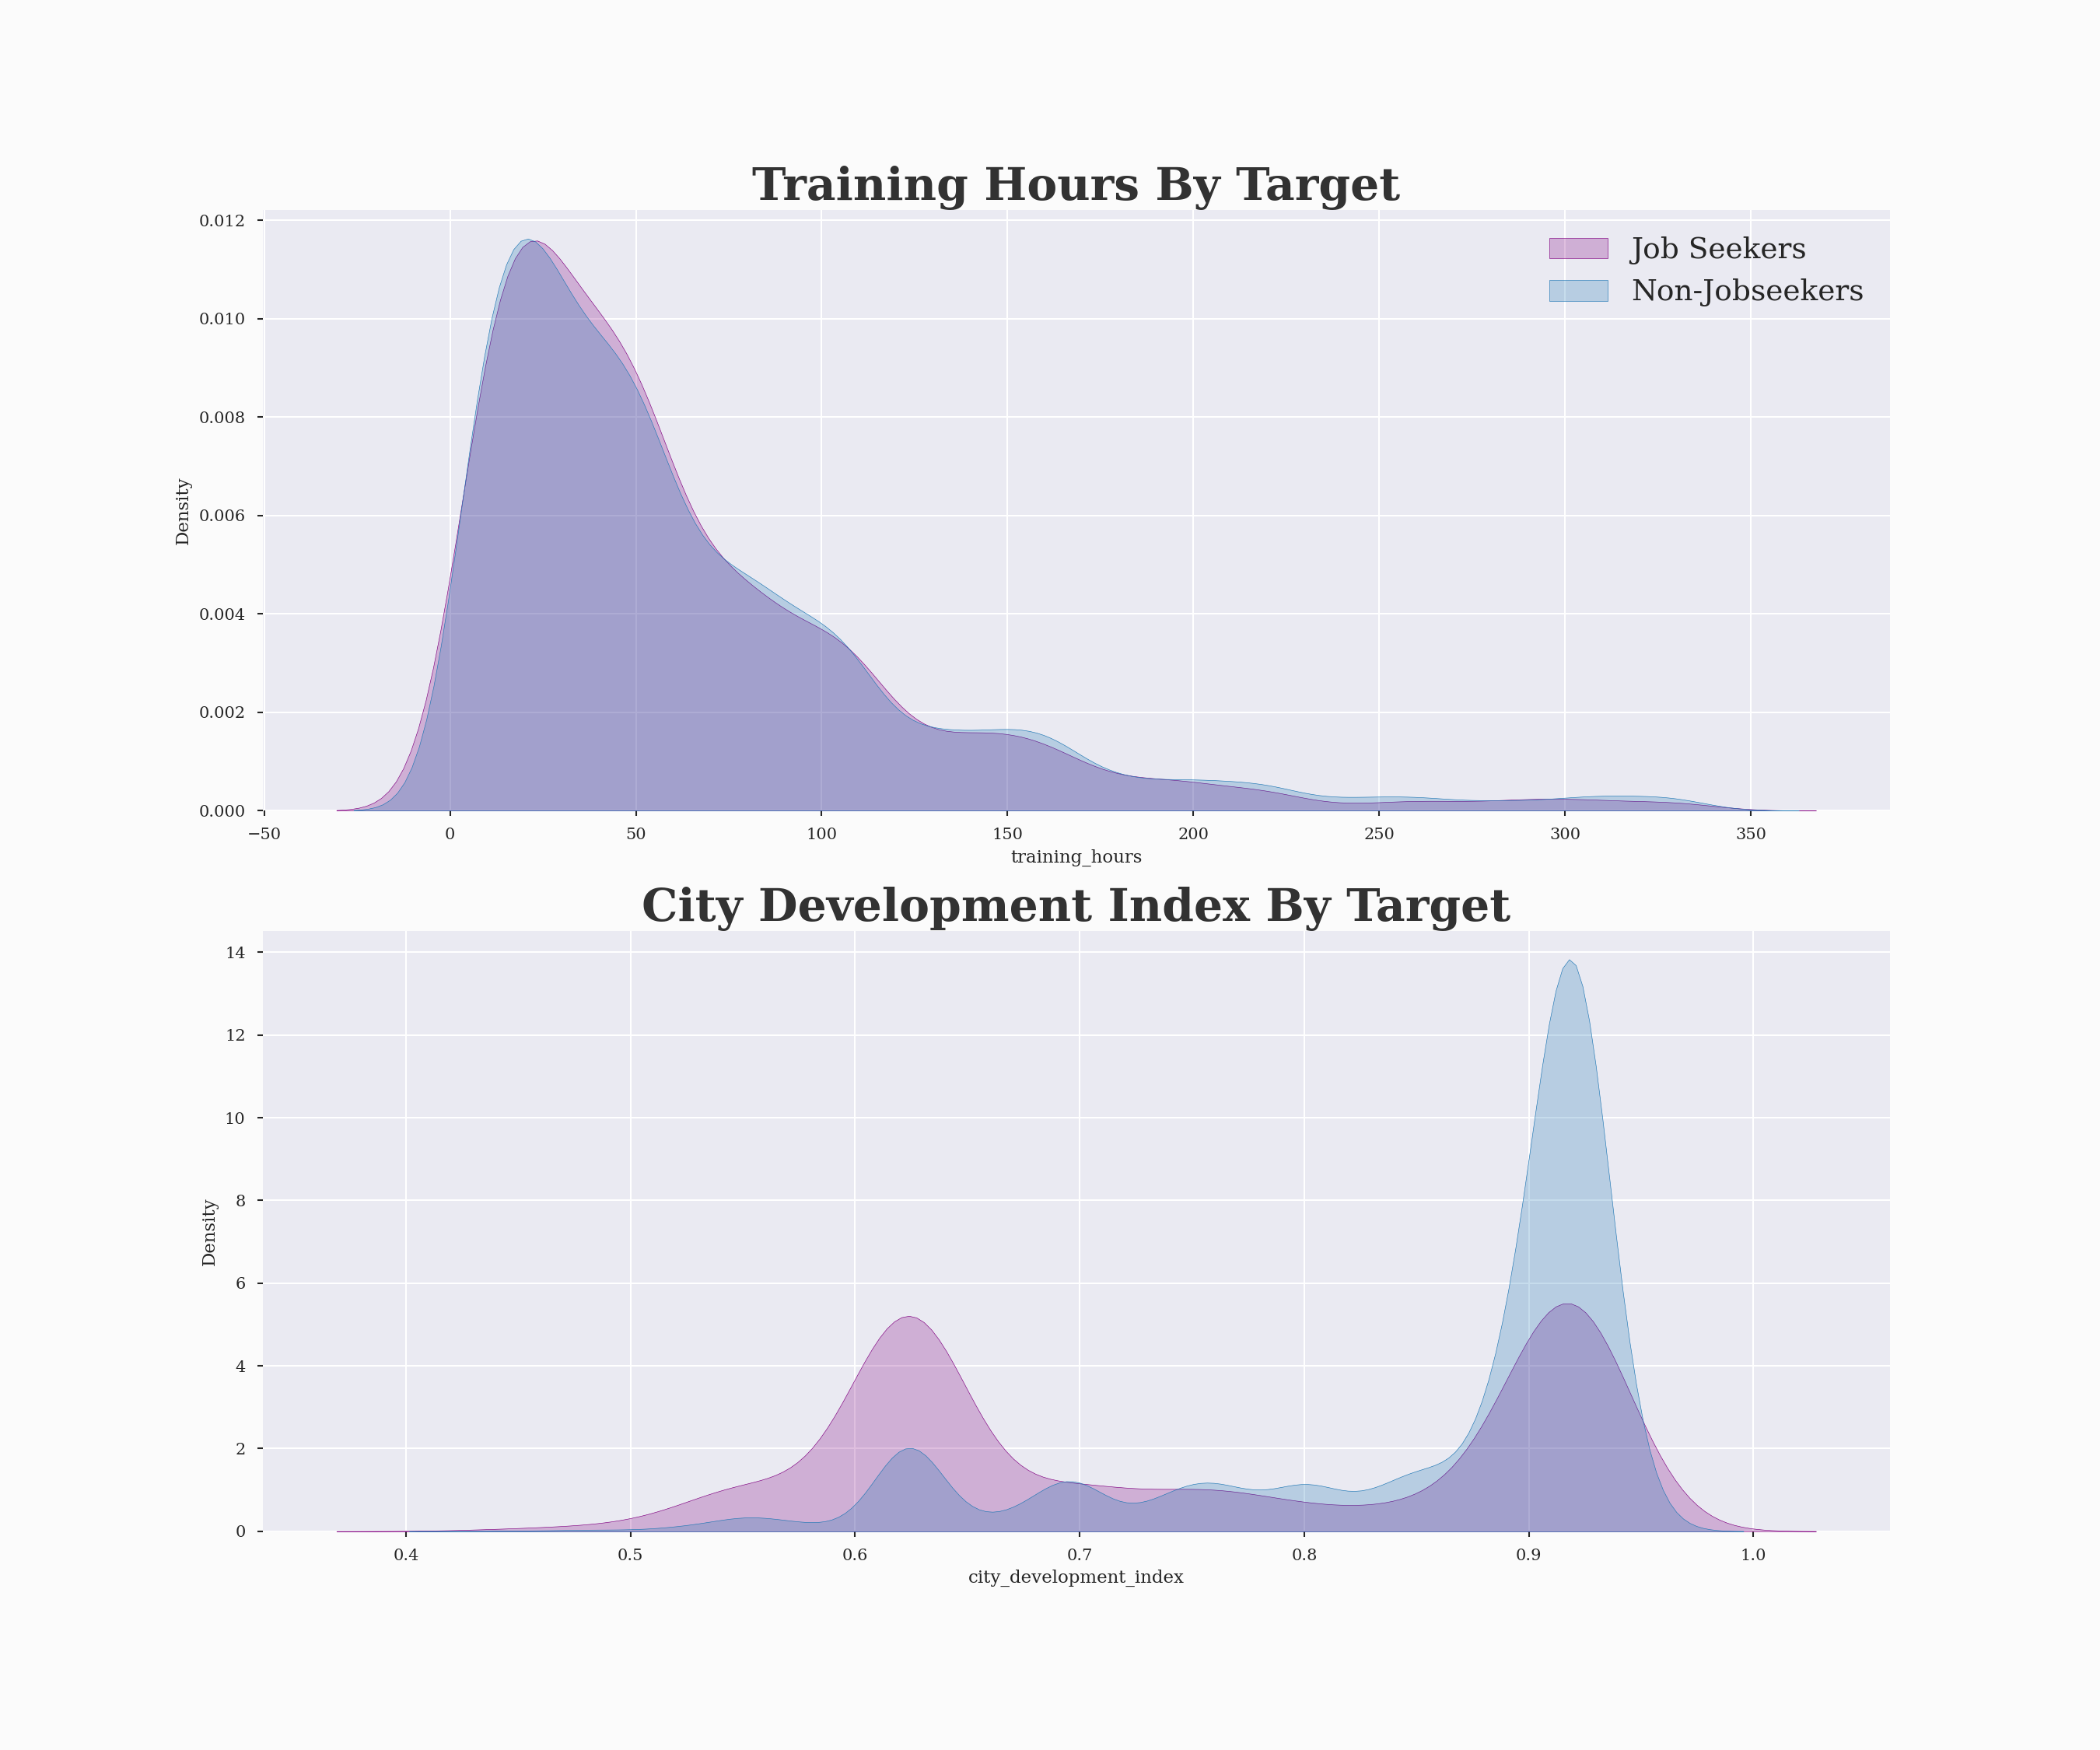
\includegraphics[width=0.45\textwidth]{continuous_distributions_target}
\end{wrapfigure}

While job seekers and non-job seekers share similar distributions on many features, there are several key differences that might provide some insight on factors that motivate candidates to search for new roles.  In particular, a smaller proportion of job seekers seem to have relevant data science experience, indicating that professionals outside of the field might be motivated to switch to careers in the growing data science industry.  Similarly, job seekers are much more likely to be full-time students looking for positions after graduation.  This might also explain why many job-seekers do not supply information about their current company since they may not be currently employed. The gender distribution between candidates actively searching and those who are not appear roughly the same, with a slighter greater share of applicants not reporting their gender.  In general, job seekers are also less experienced than their peers not on the job market and if employed, have been in the current role for 4 years or longer. 

Interestingly, job-seekers 








 

The output of this ADS comes from a logistic regression model that was trained on a synthetically upsampled data set to correct for imbalance in the target variable.  While the output of the machine learning model is a probability of the candidate being on the job market, the output of this ADS is a class label (either `Job Seeking' or `Not Job Seeking') that assumes that candidates with predicted probabilities above a threshold of 0.5 are looking for a job.




\pagebreak

\section{Implementation and Validation}

The ultimate model used for this ADS is a logistic regression trained on a dataset that was augmented using the Synthetic Minority Oversampling Technique (SMOTE).  Prior to training the model however, the creator made several choices pertaining to the preparation and pre-processing that ultimately impacted the algorithm's results.

Given the prevalence of missing values in the dataset, the imputation technique used might significantly change the distribution of our training set.  In this instance, the creator choose to handle missing values for `company\_type', `major\_discipline', and `gender' by treating them as a separate class altogether, labeled 'Unknown` or 'Not Provided`, while missing values for `company\_size' were unilaterally imputed as 0. Any observations that had missing values outside of these features were then dropped, bringing our population down to 18,014 candidates. Given that our final model is a logistic regression, and therefore sensitive to null values, it is usually appropriate to handle imputations this way.

In addition to imputing null values, the creator took several steps to prepare features before training any models.  This involved creating dummy variables for each of our many categorical variables and removing the target and unique identifier.  This expands our dataset to 190 features. For the purposes of future validation, the population is then split into test and train datasets at a 30/70 ratio.  No validation set was held out for hyper-parameter tuning.  Finally, in nearly all model pipelines, the creator scaled features through Z-score normalization, an important pre-processing step for many algorithms especially logistic regression.  From our analysis of distributions above, we see that the continuous variables in this dataset are rarely normally distributed although we make the assumption that they are in z-standard normalization.

Given the large imbalance of job seekers to non-jobseekers in this data set (25\% to 75\% respectively), the creator employs Synthetic Minority Oversampling Technique (SMOTE) to solve for this problem and improves model performance.  SMOTE is one of the most commonly used oversampling methods that aims to balance by randomly increasing minority class examples by replicating them. The technique synthetically generates new instances of the minority class from existing instances of the class by linear interpolation.  These synthetic training records are generated by randomly selecting one or more of the k\-nearest neighbors for each example in the minority class.  A randomly selected neighbor is chosen and a synthetic example is created a random point between the two existing examples in feature space.  We can replicate this procedure as many times as necessary to create class balance.  In the case of our human resources dataset, we generated over 6,000 new samples and increased the training dataset by roughly 50\%.
This approach is generally effective since it ensures that the new synthetic examples are plausible and relatively close, in feature space, to the existing observations of the minority class.  

Despite its widespread use and broad adoption of the technique for class balancing, the effect of such strategies on model fairness is largely unknown and is an undergoing area of research. In their 2020 CIKM presentation, Yan et al. demonstrated that popular balancing techniques contribute to greater differences of statistical parity, equal opportunity and equalized odds when applied to the COMPAS decision system. SMOTE, in particular, created the greatest disparity in fair outcomes of any other technique tested. By only balancing on the target variables, they argue, traditional class balancing techniques do not consider the distribution of sensitive attributes when creating synthetic samples and therefore have the potential to exacerbate unfairness towards underrepresented groups. In the context of our job seeking algorithm, for example, we could imagine seeing an over\-representation of candidates in the upsampled dataset who do not have relevant experience given the difference in distributions of experienced candidates between target classes. Similarly, we might observe an over-representation of candidates who did not provide their gender and conversely an under-representation of candidates who identify as male.  New techniques have been introduced such as 
fair class balancing and FAIR-SMOTE that begin to address some of these inequalities however they were not applied in the creation of this ADS.

After preparing a training dataset, the author ran a series of classification machine learning models (Support Vector Classification, a Decision Tree, Random Forrest, Logistic Regression and a KNN-algorithm) and evaluated the performance of each prior to deciding on a final model.  The 
performance measures that were evaluated included Accuracy, Recall, Precision and ROC Area under the curve. All of the classification models performed significantly better when trained on the SMOTE upsampled training data set.  While the author did not specify which they were optimizing for specifically, one could imagine favoring models with higher precision or recall depending on the time and investment associated with inviting a candidate to interview.  In the end, the logistic regression was chosen for its dramatically higher recall score and high overall accuracy.


\pagebreak

\section{Outcomes}

Now, we will examine the bias and fairness of the ADS by evaluating its performance across subpopulations. In particular, we examine five attributes: gender, education level, relevant experience, general experience, and city development. Given the context of our task, we consider the following metrics:
\begin{itemize}
\item Sample size, which we use to measure the balance of the dataset.
\item Selection rate, which is the portion of predicted labels matching the ‘good’ outcome. In this case, the 'good' outcome is being a "job seeker". This is because companies will often provide extra benefit to those of their employees seeking new jobs in attempts to keep them from leaving. The job seekers will also receive more job opportunities if other companies were to obtain this information. We choose this measure to whether one group receive disproportionately more "good" outcomes than others.
\item Accuracy, which is defined as $\frac{TP + TN}{P + N}$. We choose accuracy as a standard measure of the model's performance in subgroups. 
\item False Negative Rate (FNR), which in this context is the percentage of job-seekers that are predicted to be not job-seeking. We care about FNR because the false negative cases represent a lost benefit: those who could have gotten job opportunities or higher chance of promotion did not get them. The term is defined as $\frac{FN}{FN + TP}$.
\item False Positive Rate (FPR), which is the percentage among non-job-seekers that were predicted to be job-seeking. This means those who are not seeking new jobs receive potential promotion, which is a plus, and job opportunities, which might or might not be an annoyance. The companies, on the other hand, waste resources in trying to keep people who don't want to leave in the first place, hence t would be in the interest of the companies using the ADS to reduce FPR. The term is defined as $\frac{FP}{FP + TN}$.
\item Average Precision, which summarizes a precision-recall curve as the weighted mean of precision achieved at each threshold, with the increase in recall from the previous threshold used as the weight.
\item ROC AUC score, which computes the Area Under the Receiver Operating Characteristic Curve (ROC AUC) from prediction scores. We choose both Average precision and ROC score as additional measures of the accuracy. 
\end{itemize}
The baseline values for these data are as follows:

\begin{table}[h]
\centering
\begin{tabular}{ |p{3cm}||p{3cm}|}
 \hline
 Measure 		& Baseline Value\\
 \hline

sample size 	& 5405 \\

selection rate 	& 0.348566 \\

FNR 	& 0.256569\\

FPR & 0.224276 \\

accuracy		 & 0.767993 \\
average precision & 0.441032 \\
ROC score & 0.759577 \\

 \hline
\end{tabular}
\end{table}


The first protected attribute we examine is gender, which is a categorical variable with values ``Female", ``Male", ``Others", and ``Not provided". For the sake of readability, we leave all the diagrams in the appendix. As mentioned in previous section, there are disproportionately many men in the data. Nevertheless, the model doesn't have a significant gender bias. All measures demonstrate reasonable parity across gender groups.

Next, we examine education level, which is correlated with socioeconomic status. The categorical values comprise 'Primary School', 'High School', 'Graduate', 'Masters', and 'PhD', where we assume ``Graduate" to indicate "college graduate". The data is, again, imbalanced, with significantly more ``Graduate" and ``Masters" than any other education level. We observe that "graduate" have both the highest selection rate and the highest FPR, indicating that the ADS is highly likely to label ``Graduate" as job-seekers. On the other hand, those with "High School" education level have the lowest selection and FPR rate, meaning the ADS is highly likely to label them as non-job-seekers. The accuracy for the two groups are similar, meaning that there is some truth to "Graduate" having a higher likelihood to be seeking jobs and the same for those with high school diplomas. Nevertheless, this means those with high school diplomas will potentially receive less job opportunities (if the ADS is used by other companies) and chance of promotion (if the ADS is used by the current company).

Then, we examine relevant experience, which is a binary variable containing either ``yes" or ``no". We observe that the selection rate and FPR for those with no job experience are about twice as much as that of those with job experience, indicating that the ADS has the tendency to label those with no relevant job experience as ``job seekers". This hurts job seekers with relevant experience because they are less likely to be viewed as job-seeking, hence receive less opportunities as a result.

Furthermore, we examine experience in general, which correlates with age. Recall that in previous section, we changed the years in experience of everyone with more than 20 years of experience to 20. We observe that the more experience a person has, the less likely the ADS will think they are job-seeking. The Selection rate and the FPR for those with no experience is almost three times as high as the values for those with 20 or more years of experience. This bias put older people at a disadvantage. Since they are not viewed as job-seeking, they will miss out on job opportunities and potential promotion.

Lastly, we examine the development index of the city that the data scientist currently resides. The index is calculated base on five sub indices: infrastructure, waste, health, education and city product. We observe that the selection rate and FPR for cities with development index less than 0.6 is almost 1, meaning that being in such a city make the ADS automatically label one as a "job-seeker". The lower accuracy for those cities help us discern that this is more likely a bias than a fact. Such a bias will bring benefits to those living in those relatively less developed cities. On the other hand, companies will waste resources as a result and potentially loss employees in more developed cities due to the high FNR. 

Besides the previously mentioned measure, we also calculated the demographic parity ratio and the equalized odds ratio to further evaluate the fairness of the ADS. The demographic parity ratio is defined as the ratio between the smallest and the largest group-level selection rate, across all values of the sensitive feature(s). The demographic parity ratio of 1 means that all groups have the same selection rate. Equalized Odds Ratio is the smaller of two metrics: true positive rate ratio and false positive rate ratio. The equalized odds ratio of 1 means that all groups have the same true positive, true negative, false positive, and false negative rates.The results are the follow:
\begin{table}[h]
\centering
\begin{tabular}{ |p{4cm}||p{3cm}||p{3cm}|}
 \hline
Sensitive Attributes 		& Demographic Parity Ratio & Equalized Odds Ratio\\
 \hline

gender 	& 0.80 & 0.69 \\

education level 	& 0.12 & 0.00\\

relevant experience 	& 0.57 & 0.48\\

experience & 0.18 & 0.18\\

city development		 & 0.19 & 0.13\\

 \hline
\end{tabular}
\end{table}

\pagebreak

\section{Conclusion \& Summary}
\begin{itemize}
\item Do you believe that the data was appropriate for this ADS?  
\item Do you believe the implementation is robust, accurate and fair?  Discuss any choice of accuracy and fairness measures and explain which stakeholders may find these measures appropriate.
\item Would you be comfortable deploying this ADS in the public sector, or in industry?  Why so or why not?
\item What improvements do you recommend to the data collection, processing or analysis methodology?
\end{itemize}


All of the code and analysis for this report can be found \href{https://github.com/cas2247/RDS_Algorithmic_Fairness}{here}.


\begin{thebibliography}{9}


\bibliography{\jobname}

\bibitem{10.1145/3468264.3468537}Chakraborty, J., Majumder, S. \& Menzies, T. Bias in Machine Learning Software: Why? How? What to Do?. {\em Proceedings Of The 29th ACM Joint Meeting On European Software Engineering Conference And Symposium On The Foundations Of Software Engineering}. pp. 429-440 (2021), https://doi.org/10.1145/3468264.3468537


\bibitem{Chawla_2002}Chawla, N., Bowyer, K., Hall, L. \& Kegelmeyer, W. SMOTE: Synthetic Minority Over-sampling Technique. {\em Journal Of Artificial Intelligence Research}. \textbf{16} pp. 321-357 (2002,6), https:%5C/%5C/doi.org%5C/10.1613%252Fjair.953

\bibitem{joshuaswords_2021}Joshuaswords HR data visualization \& prediction. {\em Kaggle}. (April 2021), https://www.kaggle.com/code/joshuaswords/awesome-hr-data-visualization-prediction/data

\bibitem{10.1145/3340531.3411980}Yan, S., Kao, H. \& Ferrara, E. Fair Class Balancing: Enhancing Model Fairness without Observing Sensitive Attributes. {\em Proceedings Of The 29th ACM International Conference On Information \& Knowledge Management}. pp. 1715-1724 (2020), https://doi.org/10.1145/3340531.3411980

\end{thebibliography}




\bibliographystyle{abbrv}
% \bibliography{references}  % need to put bibtex references in references.bib 
\end{document}